\chapter{Detecting Abnormalities in Materials Data}  \label{chap:pyqalloy}


\section{Introduction} \label{pyqalloy:sec:intro}

\todo

\begin{figure}[H]
    \centering
    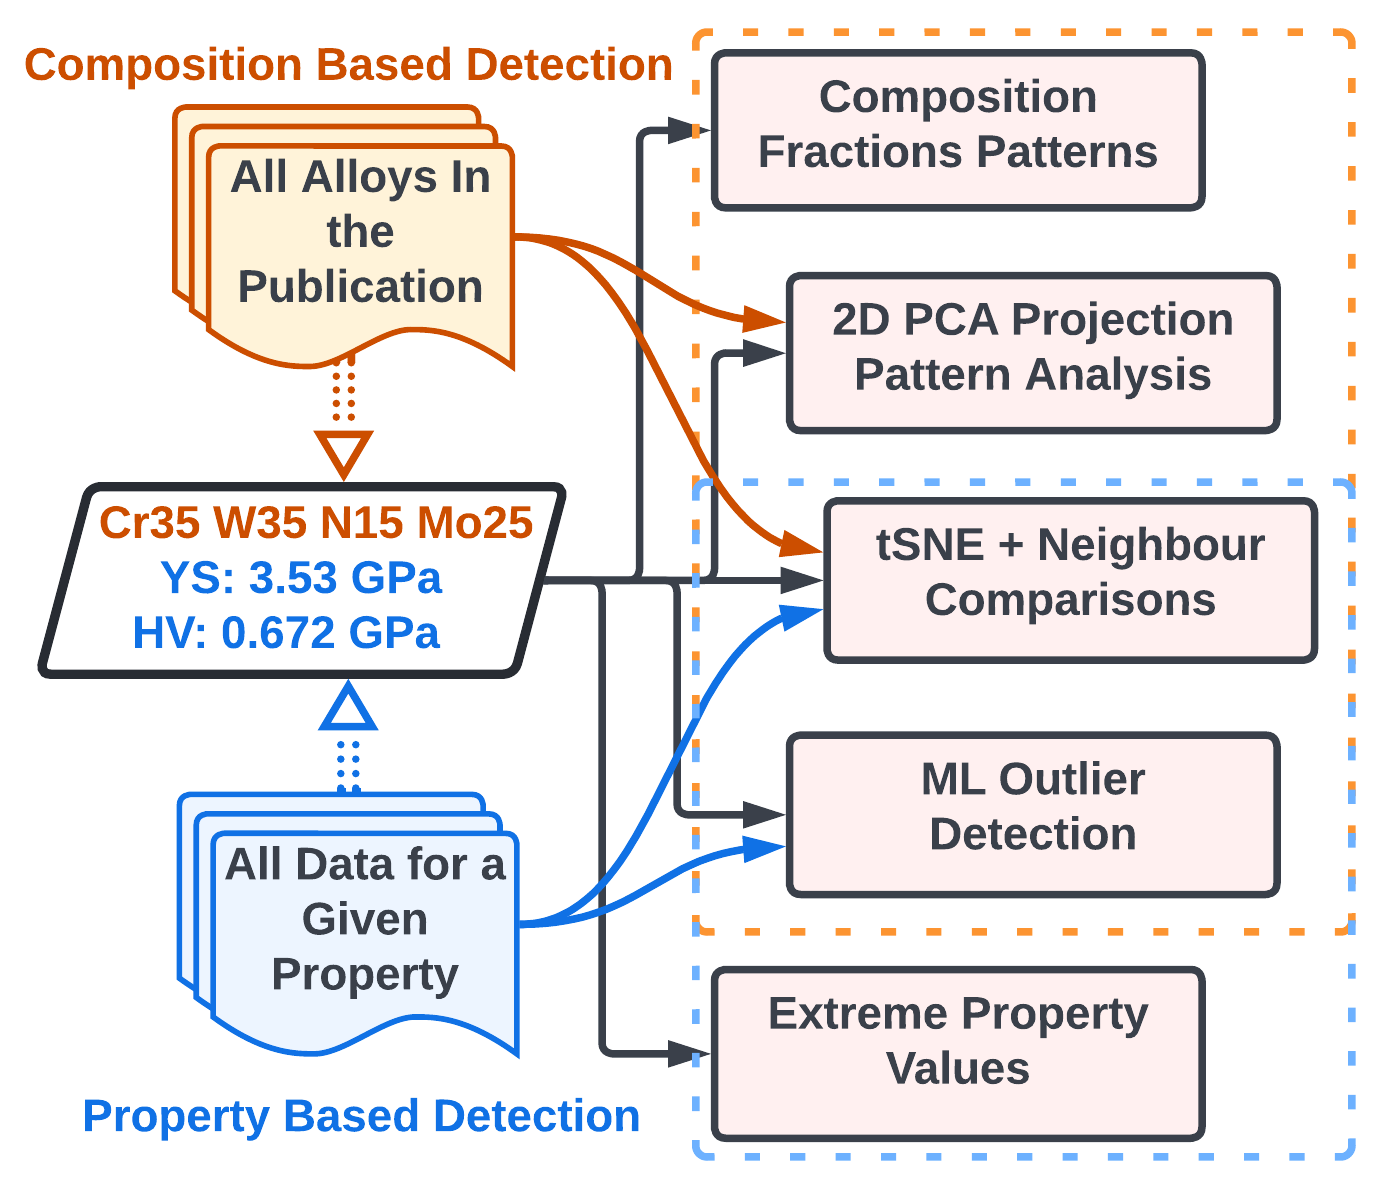
\includegraphics[width=0.6\textwidth]{pyqalloy/AbnormalCompositionDetection_v1.png}
    \caption{Schematic of \texttt{PyQAlloy} software operating in several contexts to detect and investigate common abnormalities discussed in Subsections \ref{pyqalloy:ssec:extreme} through \ref{pyqalloy:ssec:global}.}
    \label{pyqalloy:fig:schematic}
\end{figure}

\section{Common Abnormalities and Detection of Errors} \label{pyqalloy:sec:abnormalities}


\subsection{Extreme Values} \label{pyqalloy:ssec:extreme}

\todo

\begin{figure}[H]
    \centering
    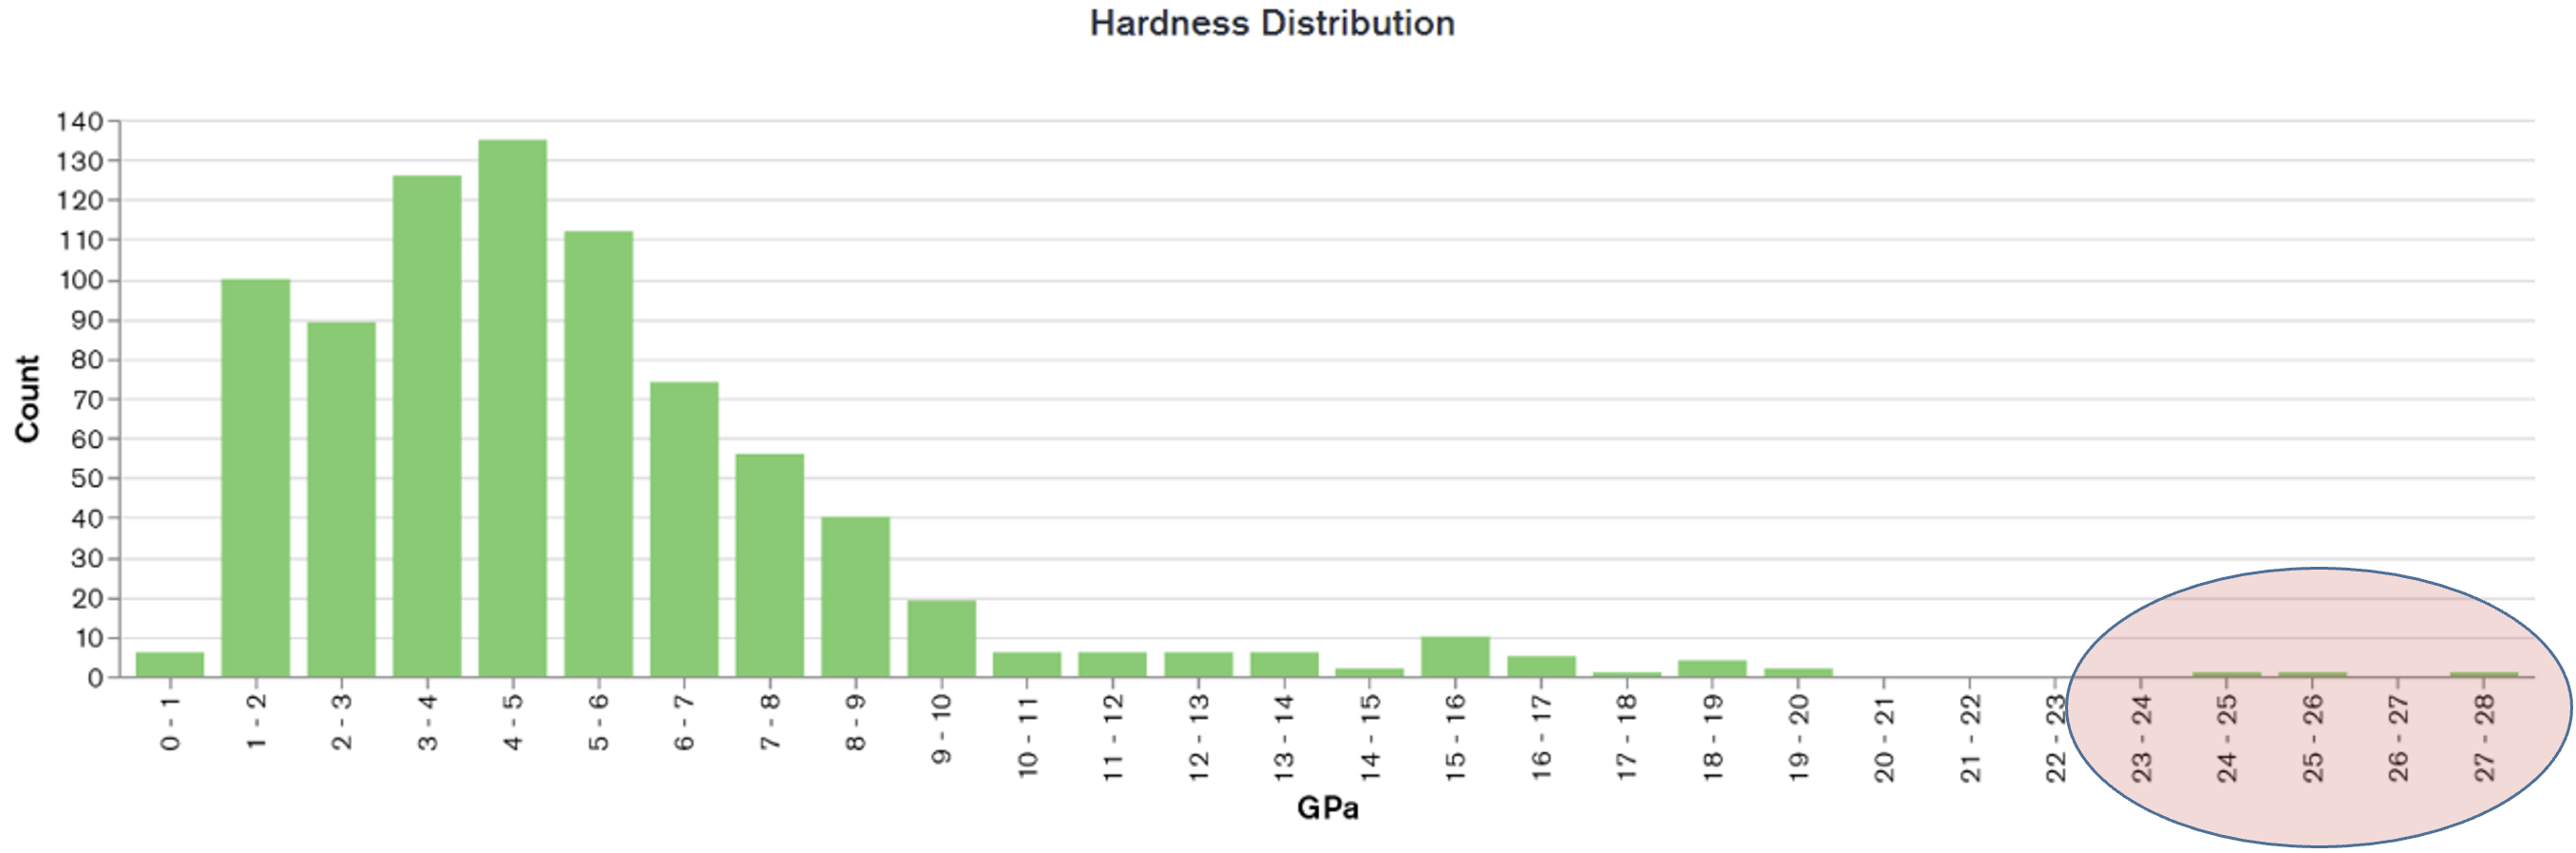
\includegraphics[width=0.95\textwidth]{pyqalloy/pyqalloy_extremevalues.png}
    \caption{A legacy, pre-curation ULTERA hardness data histogram. The extreme, out of distribution values (highlighted) indicate possible misinterpretation. Two out of three were misreported due to "extra 0" typo, while the highest one (27.5 GPa) was properly reported \ch{Mo_{40.5}Ni_{40.5}B_{10}Si_9} extremely hard metallic glass \cite{Kim2016DevelopmentRatios}. Similar analysis applies to extremely low values.}
    \label{pyqalloy:fig:extreme}
\end{figure}


\begin{figure}[H]
    \centering
    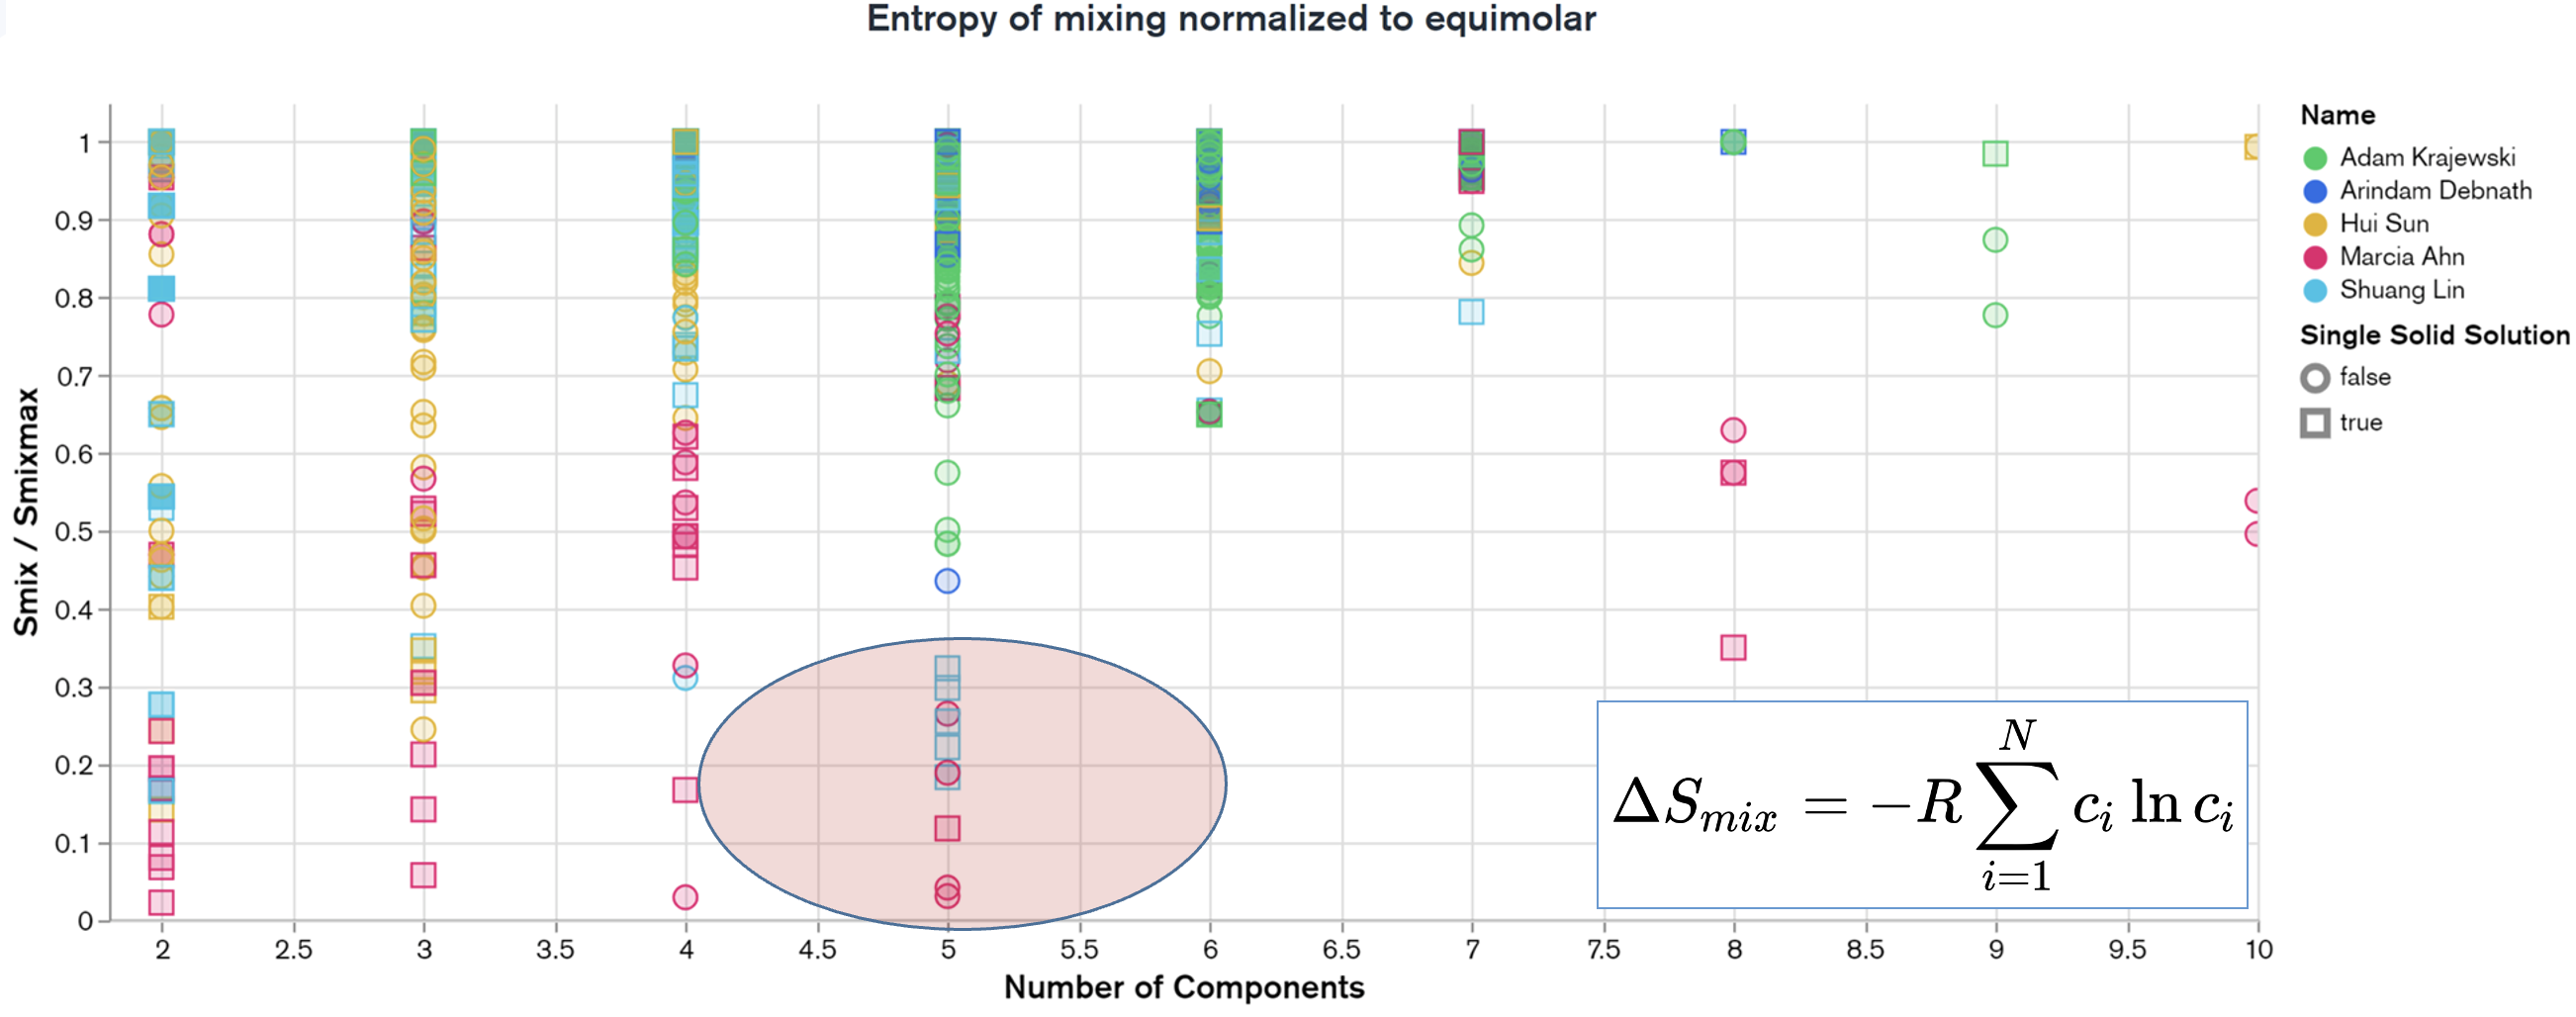
\includegraphics[width=0.95\textwidth]{pyqalloy/pyqalloy_entropy.png}
    \caption{An example of extreme value detection in secondary data characteristics relative to expectations. The legacy, pre-curation ULTERA data plot of ideal mixing entropy of a given alloy divided by the maximum ideal mixing entropy corresponding to the number of components present (value of $1$ indicates equimolar alloy). Extremely low values in this metric indicate high likelihood of "double click" or "missing comma" typos at data parsing which resulted in one element becoming highly dominant.}
    \label{pyqalloy:fig:lowentropy}
\end{figure}


\subsection{Single Composition Patterns} \label{pyqalloy:ssec:singlecomp}

\todo



\subsection{Single Study Patterns}   \label{pyqalloy:ssec:singlestudy}

\todo

\begin{figure}[H]
    \centering
    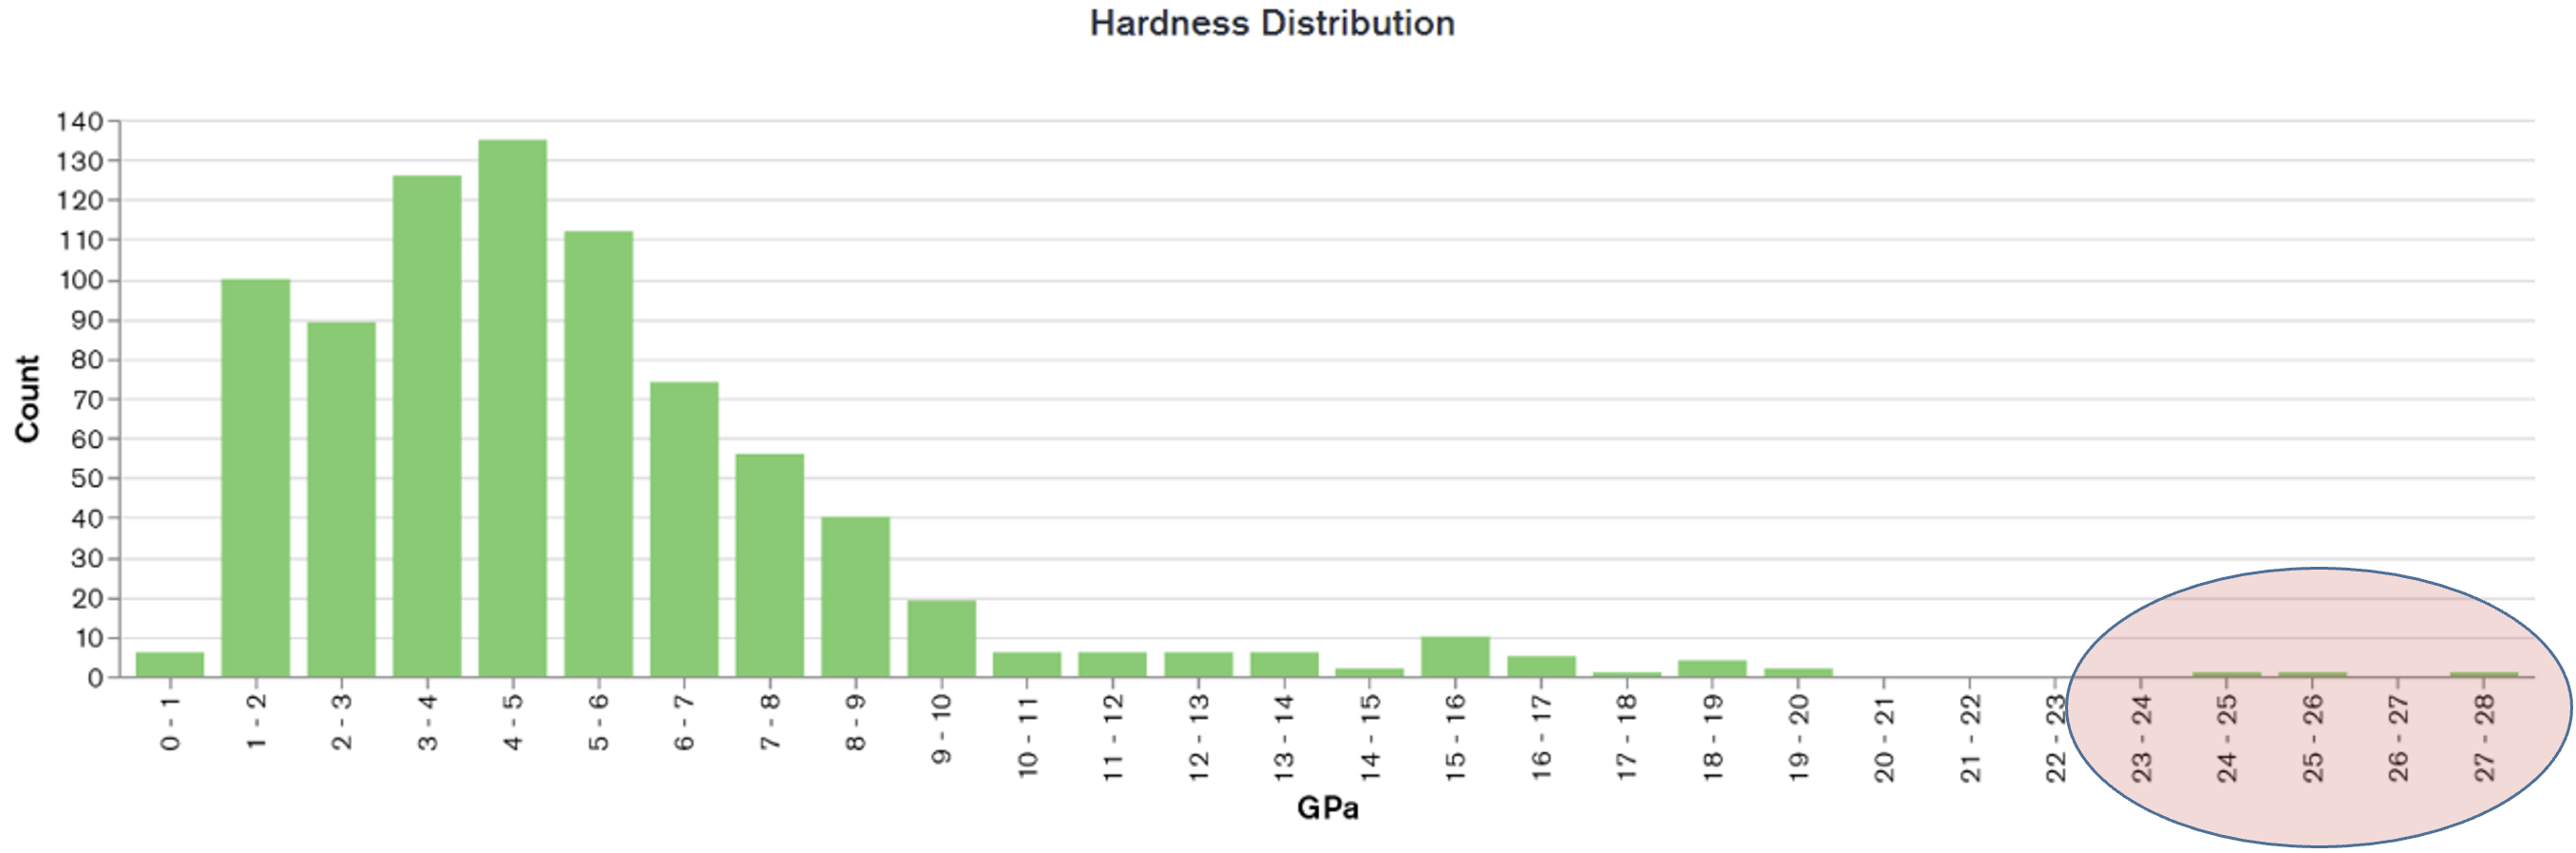
\includegraphics[width=0.95\textwidth]{pyqalloy/pyqalloy_extremevalues.png}
    \caption{Expected patterns in the PCA projections of high entropy alloy composition vectors onto a 2D plane common for vast majority of alloy design studies which either (left) take an alloy and progressively modify it through elemental substitutions or mixing with another alloy in one or more ways, resulting in one or more linear patterns, or (right) test many different elemental combinations that are thought to possibly work well in the application in a anti-systematic fashion (in chemical space) does not follow any lower dimensional pattern and results in a point cloud. Breaks in these patterns, like out-of-line points or anisotropic point clouds indicate possible errors and should be screened.}
    \label{pyqalloy:fig:expectedpatterns}
\end{figure}



\begin{figure}[H]
    \centering
    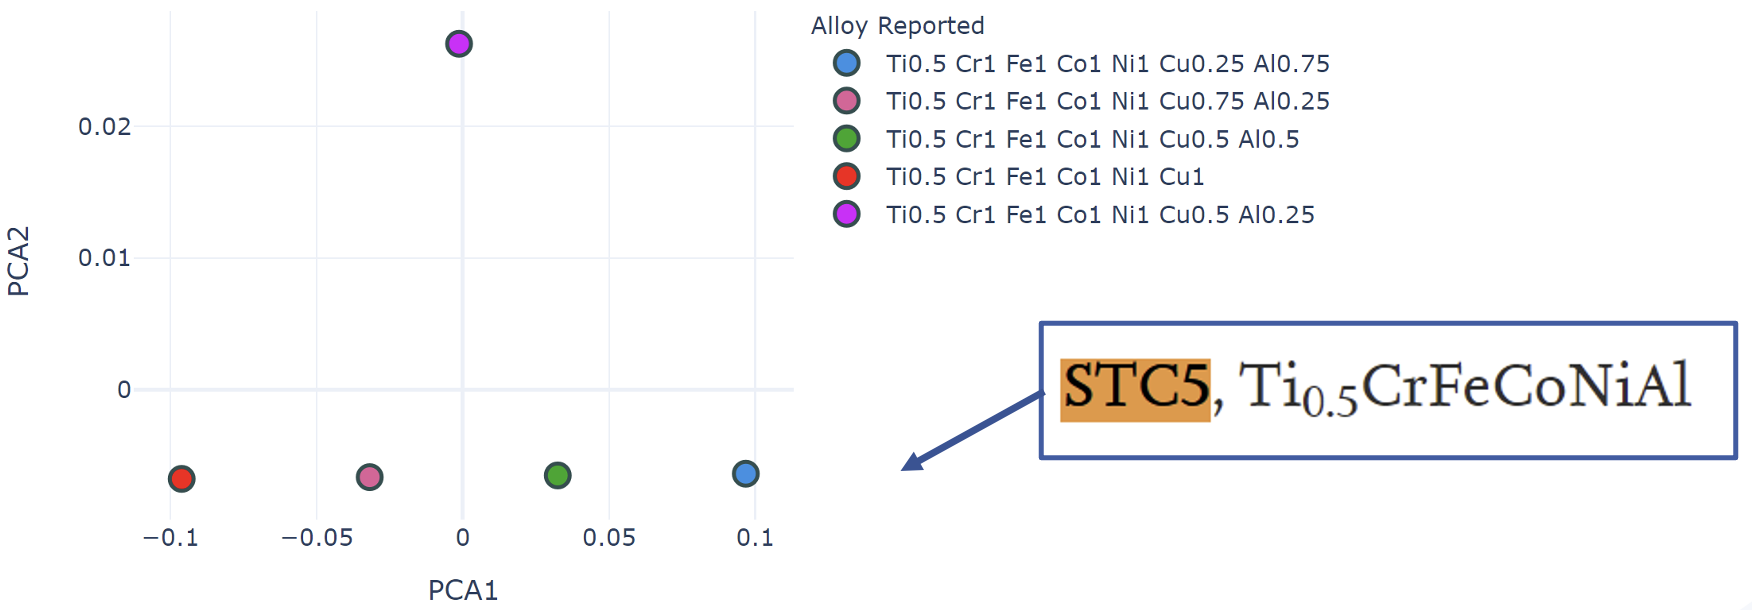
\includegraphics[width=0.95\textwidth]{pyqalloy/pyqalloy_HumanError.png}
    \caption{An example of out-of-line pattern detected in a literature review study. It was caused by the researcher parsing a publication incorrectly noting the composition relative to the source \cite{Wang2009AtomicAlloy}. Composition similar to other points makes it look right; thus, such errors are nearly impossible to catch using other methods.}
    \label{pyqalloy:fig:patternbreak1}
\end{figure}




\begin{figure}[H]
    \centering
    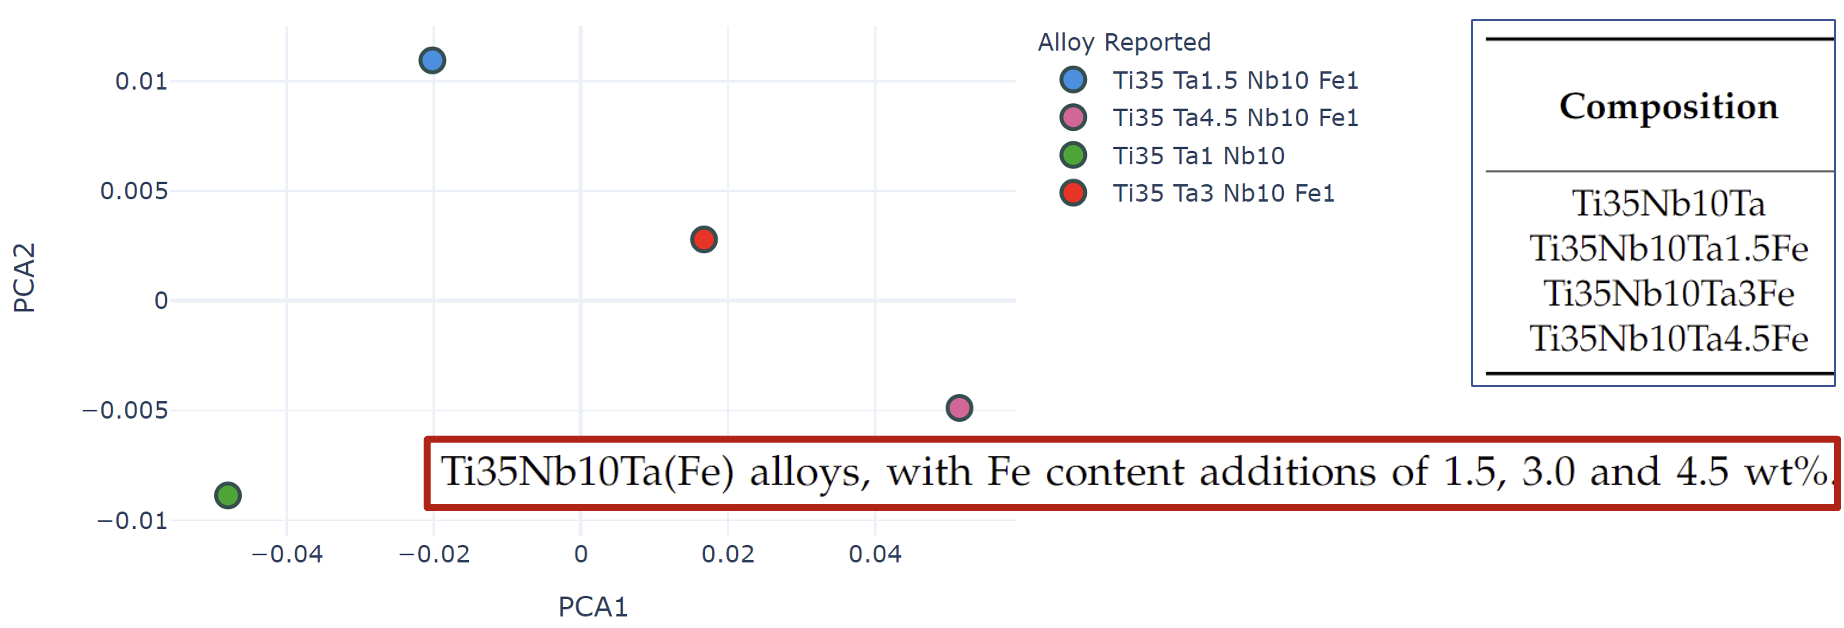
\includegraphics[width=0.95\textwidth]{pyqalloy/pyqalloy_CompositionNotation.png}
    \caption{An example of out-of-line pattern detected in a literature review study, in which chemical formulas present in the source publication \cite{Amigo2019MechanicalApplications} are correctly parsed. However, they are shorthand composition notations rather than actual chemical formulas of the studied material and need to be interpreted; thus, they are incorrectly reported. Such misinterpretations typically follow some incorrect patterns locally but fail to do so if any component is removed or added to the mix as depicted here.}
    \label{pyqalloy:fig:patternbreak2}
\end{figure}



\subsection{Global Patterns} \label{pyqalloy:ssec:global}

\todo

\begin{figure}[H]
    \centering
    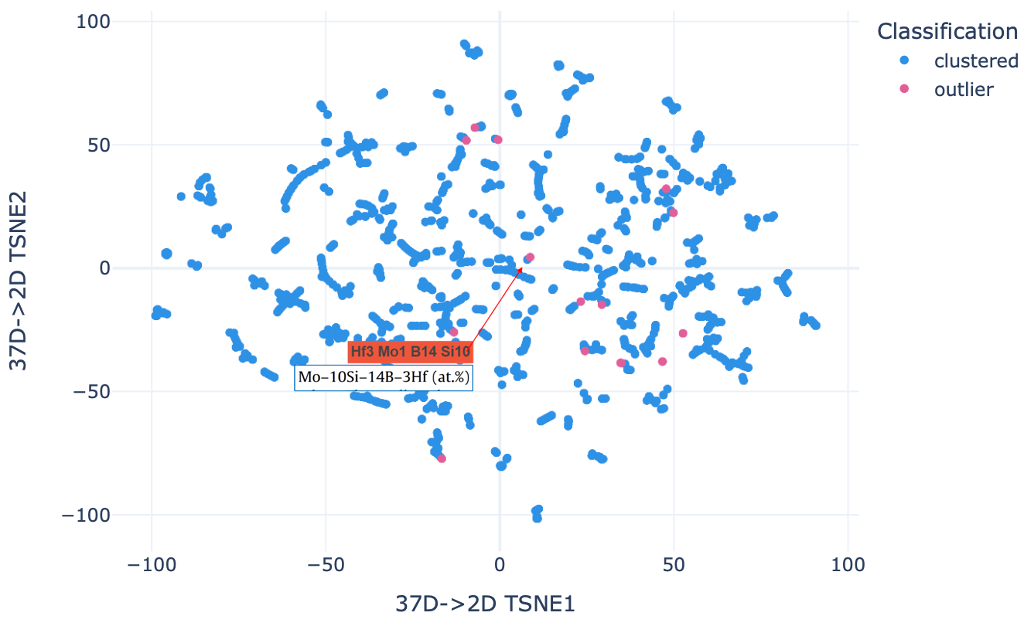
\includegraphics[width=0.95\textwidth]{pyqalloy/PyQAlloy_tSNE+DBSCAN.png}
    \caption{2D tSNE embedding of all chemical compositions present in ULTERA based on alloy neighborhoods, overlaid with outliers detected through DBSCAN method operating in the high-dimensional real composition space. Singular outliers between tSNE clusters are expected and indicate novel compositions, while outliers within clusters indicate far removed members of an alloy family which are likely incorrect. The highlighted \ch{B-Hf-Mo-Si} alloy is close to other alloys in that system but fraction of \ch{Mo} was omitted by the parsing researcher. In the depicted case, abnormality was not detected by lower level methods because only one alloy was reported.}
    \label{pyqalloy:fig:patternglobal}
\end{figure}





\section{Software Implementation} \label{pyqalloy:sec:software}

\todo









\printbibliography[heading=subbibintoc]